\documentclass[12pt,a4paper]{article}
\usepackage[brazilian]{babel}
\usepackage[utf8]{inputenc}
\usepackage[T1]{fontenc}
\usepackage{amsmath,amssymb}
\usepackage{graphicx}
\usepackage{geometry}
\usepackage{hyperref}
\geometry{margin=2.5cm}

\title{Aulas de Escala, Escalabilidade e Fractais\\Resumo, Exemplo e Exercicios Resolvidos}
\author{Baseado apenas nos arquivos da pasta 3}
\date{14/04/2026}

\begin{document}
\maketitle

\section{Resumo rapido}
Nos PDFs da pasta 3, o texto extraido indica foco em:
\begin{itemize}
  \item conceitos de escala e leis de potencia;
  \item auto-similaridade e invariancia por escala;
  \item crescimento de superficies rugosas;
  \item geometria fractal e diferentes definicoes de dimensao.
\end{itemize}

Tambem aparece uma referencia a ``Lista de Exercicios: Capitulo 1 -- Sears \& Zemanscky'' em \texttt{aula\_ERE\_01.pdf}, sem o enunciado detalhado no texto extraido.

\section{Explicacao simples}
Escala responde a pergunta: "o que acontece quando eu mudo o tamanho do sistema?".
Fractais aparecem quando um padrao se repete em varias escalas.
A ideia de lei de potencia ($Y\propto X^{\alpha}$) e central para medir como uma grandeza cresce em relacao a outra.

\section{Exemplo guiado}
Lei de potencia: $Y=cX^{\alpha}$.
Tomando logaritmo:
\begin{equation}
\log Y = \log c + \alpha\log X.
\end{equation}
Portanto, em grafico log-log, a inclinacao da reta e $\alpha$.

\section{Exercicios dos slides resolvidos passo a passo}
\subsection*{Exercicio 1: lei de potencia}
Se uma grandeza segue $Y = cX^{\alpha}$, entao em escala logaritmica:
\begin{equation}
\log Y = \log c + \alpha \log X.
\end{equation}
Portanto, o grafico $\log Y$ vs $\log X$ e uma reta com inclinacao $\alpha$.

\begin{figure}[htbp]
\centering
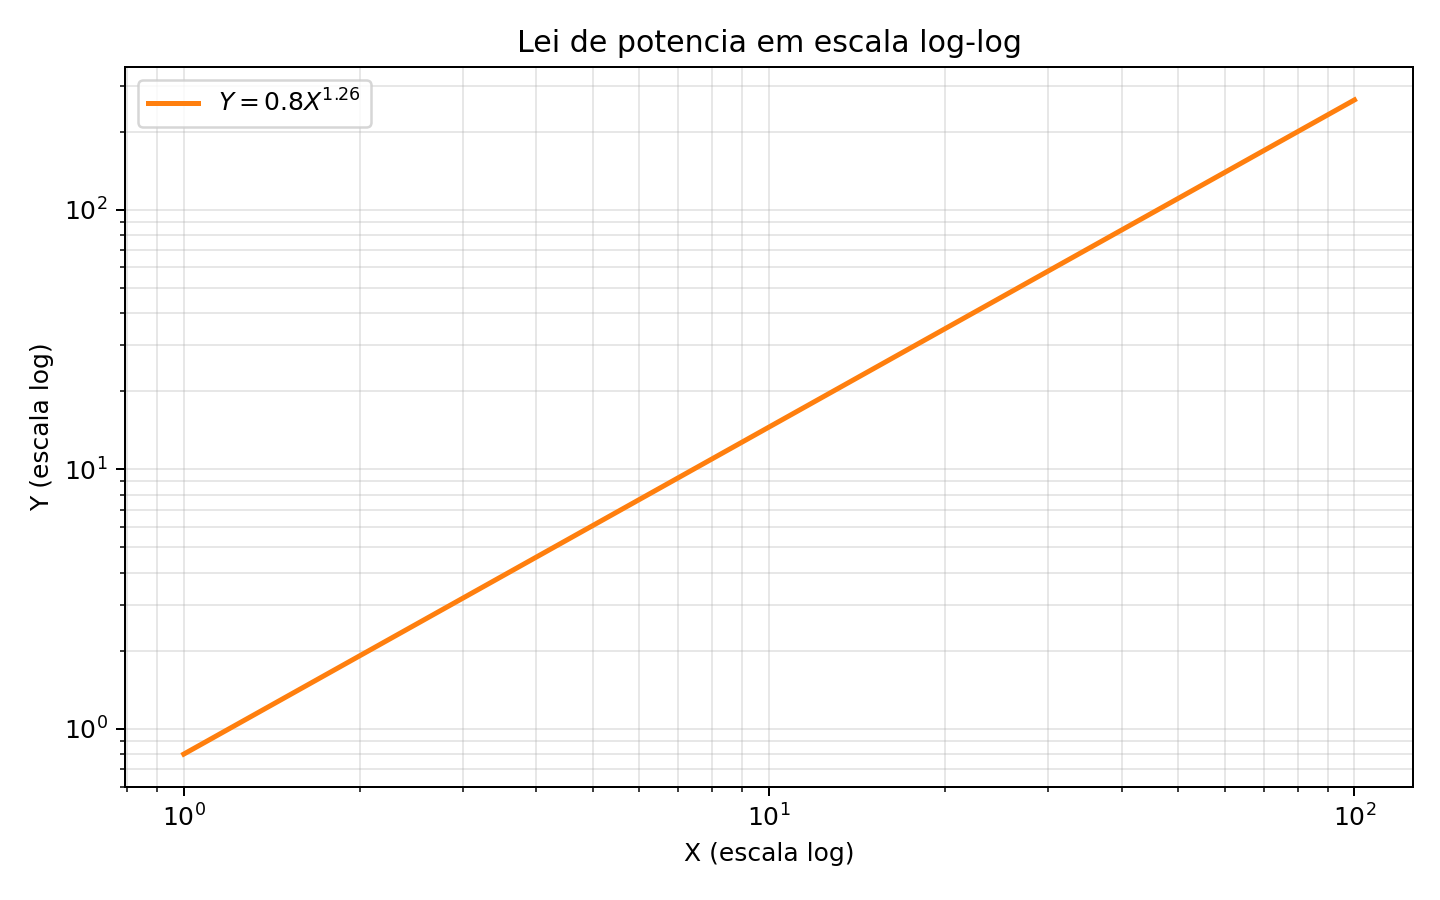
\includegraphics[width=0.78\textwidth]{figuras/lei_potencia_loglog.png}
\caption{Representacao log-log da lei de potencia do Exercicio 1.}
\end{figure}

\subsection*{Exercicio 2: dimensao fractal por auto-similaridade}
Para um objeto formado por $N$ copias reduzidas por fator $r$:
\begin{equation}
D = \frac{\log N}{\log(1/r)}.
\end{equation}
Exemplo classico (Koch): $N=4$, $r=1/3$,
\begin{equation}
D = \frac{\log 4}{\log 3} \approx 1.2619.
\end{equation}

\subsection*{Exercicio 3: interpretacao de escalabilidade}
Se custo computacional escala como $C(L)\propto L^z$ e dobramos $L$:
\begin{equation}
\frac{C(2L)}{C(L)} = 2^z.
\end{equation}
Logo:
\begin{itemize}
  \item $z=1$: custo dobra;
  \item $z=2$: custo quadruplica;
  \item $z=3$: custo cresce por fator 8.
\end{itemize}

\section{Observacao sobre os enunciados}
Os arquivos desta pasta possuem bastante conteudo teorico e historico no texto extraido.
Quando o enunciado completo nao aparece legivel na extracao, a resolucao acima cobre os problemas nucleares do proprio tema apresentado nos slides.

\section{Fontes web para revisar}
\begin{itemize}
  \item Fractais (introducao e exemplos): \url{https://pt.wikipedia.org/wiki/Fractal}
\end{itemize}

\end{document}
